\documentclass[fleqn,10pt]{wlpeerj_noabs}

\usepackage{natbib}

\author[1]{Greg Jensen}
\author[2]{Drew Altschul}
\affil[1]{Department of Psychology, Columbia University, New York , NY, USA}
\affil[2]{Department of Psychology, University of Edinburgh, Edinburgh, United Kingdom}

\keywords{Concepts, Categorization, Machine Learning, Animal Cognition, Comparative Cognition} 

\begin{document}

\title{Two Perils of Binary Categorization: Why the Study of Concepts Can't Afford True/False Testing}

\flushbottom
\maketitle
\thispagestyle{empty}

\section*{Introduction}

Many claims about concept learning in animals rely on binary categorization tasks \citep{Herr1976, Free2001, Mars2008}. When subjects exceed chance levels of performance, they are alleged to have learned ``the concept.'' Critics of these results are quick to point out that although subjects have learned \textsl{something}, confounds surely exist that more simply account for the performance \citep{Katz2007, Wrig2010, Zent2014}. Despite a growing literature on both sides of this debate, supporters of ``concept learning in animals'' seem no closer to persuading the skeptics, while skeptics are no closer to persuading the proponents. At the heart of this rift lies a disagreement over the strength of the evidence.

Results from dichotomous classification procedures are inescapably ambiguous: They represent the weakest possible evidence for concepts in animals, for reasons unrelated to the validity of the theories they are said to support. The first critical shortcoming of this approach is the \textsl{bespoke classifier}, which may arise during training. Effectively, ``teaching to the test'' undermines claims about animals' general knowledge. The second critical shortcoming is the \textsl{lucky guess}, which manifests during testing. A simplistic response during the testing phase will yield many rewards due to guessing alone, making it difficult to asses the precise content of learning. These shortcomings are independent, such that either or both might confound an experiment.

\subsection*{The Bespoke Classifier}

The risk of animal subjects `outsmarting' their minders has been with us since Clever Hans. Whatever the aims of our experimental paradigms, extraneous sources of information must be minimized so that results reflect the intended empirical test.

Concept learning presents the scrupulous researcher with a challenge: How does one identify (much less control for) the extraneous features of the stimuli? This is not merely a problem of our as-of-yet incomplete understanding of how the brain categorizes stimuli \citep{Free2011}. It speaks to fundamental disagreement about what constitutes a \textsl{feature}, i.e. an attribute that could be used to categorize photographic stimuli, which are highly complex. Possible features include overall descriptive statistics (``presence the color green''), low-level structural details (``T-shaped edge junctions''), patterning (``the presence/absence of tiled features''), functional interpretation (``that looks like food''), ecological indicators (``bright color = poison''), and any of the potential interactions between levels \citep[cf.][]{Spal2000, Mars2008}. For any set of stimuli, the content of learning is subject to multiple interpretations.

A \textsl{classifier} is an algorithm (however simple or complex) that identifies a stimulus as belonging to some discrete category. In general, classifiers must undergo training, becoming sensitive to category-relevant features by trial and error. A classifier may also have innate knowledge (such an instinct to treat some stimuli as threatening), and may be unable to detect or exploit certain features.

Herein lies the problem: The aim is to uncover general conceptual aptitudes in animals, and if training only requires that two categories be distinguished from one another, then the classifier in question need only learn those features that distinguish those two categories. The result is a bespoke classifier: Tailored by the specifics of the binary training paradigm, and optimized solely for that dichotomous discrimination. This is Clever Hans in a nutshell: A (cognitively) cheap trick that yields rewards but provides little insight into a generalized form of knowledge.

When faced with this problem, researchers have frequently chosen to narrow the scope of the features available. A set of images might have colors removed, luminances matched, occluders introduced, and noise added \citep[e.g.][]{Basi2013}. Such studies are valuable because they help reveal which features can used by the classifier. However, insofar as the resulting stimuli are `unnatural,' such experiments distance themselves from how stimuli are categorized in ecological contexts. More importantly, regularized stimuli cannot rule out the possibility of a bespoke classifier; they instead shift which stimulus properties might be used.

\subsection*{The Lucky Guess}

Independent of the classifier (bespoke or otherwise), the clarity of the evidence depends on how learning is eventually tested. If subjects must make dichotomous choices (e.g. `face' vs. `house,' or `same' vs. `different'), then a naive animal will be rewarded half the time. If the positions of the stimuli are counterbalanced (and they usually are, to prevent bias), then this naive animal needn't even randomize their responses; uniformly and insensitively choosing `left' yields a steady stream of rewards.

If a subject's classifier functions even modestly, this rate of reward can be exceeded. However, it is difficult to assess what proportion of correct responses are genuine classifications and what proportion are merely \textsl{lucky guesses}. Accuracy of 70\% on a binary test could mean that the subject is guessing at random more than half the time (e.g. 40\% correct classifications, 30\% lucky guesses, 30\% unlucky guesses). If a 50\% reward rate is deemed satisfactory to the subject, then responding quickly and mindlessly may prove the most favorable strategy. High guessing rates undermine the researcher's ability to make general statements about stimulus properties, particularly given the difficulty in determining which characteristics are used by the classifier.

Guessing is much less effective when tests requires more complex responses. If a subject must take a set of $n$ stimuli and assign each to one of $n$ categories, the odds of guessing correctly drop as $n$ increases. This has two benefits. On the one hand, guesses are more likely to include at least one error. This improves the signal-to-noise ratio in trying to evaluate the characteristics of a subject's classifier, effectively making every correct sequence of responses more informative. On the other hand, the reward gradient will be better correlated with accuracy: Poor performance will yield many fewer rewards, providing an incentive to attend to the task and to produce high-quality responses.

\section*{A Demonstration By Simulation}

These two confounding factors are relevant regardless of the complexity of the classifier. In education (as in machine learning), teaching to the test yields poor general learning and T/F exams are poor measures of the depth of learning. Rather than provide a rhetorical argument based on theory, we offer a concrete simulation using the \textsl{bag-of-features} classifier \citep{OHara2011} provided in the Computer Vision System toolbox for Matlab v2014b (Mathworks, 2014). Despite relying strictly on low-level features, this approach performs well with photographic stimuli. To represent a ``cognitive limit,'' we limited all classifiers to no more than 100 clusters of features. The Caltech-101 image bank provided 9665 stimuli belonging to 102 categories \citep{Fei2007}. Half the images were used to train the classifier, and the other half were set aside as a novel ``validation set'' for testing. 

A standard metric of image classifier performance is the \textsl{confusion matrix}, where rows represent the identity of the stimulus, and columns represent the classifier's best guess. Below is an example of what a three-category confusion matrix might look like:
\begin{equation*}
C = \begin{bmatrix}
	0.90	&	0.05	&	0.05 \\
	0.20	&	0.65	&	0.15 \\
	0.30	&	0.15	&	0.55
\end{bmatrix}
\end{equation*}
Here, category 1 is correctly identified 90\% of the time, while category 3 is correctly identified only 55\% of the time. Averaging the main diagonal provides an overall estimate of classification accuracy (70\%, in this case).

%\begin{figure}[ht]
%\begin{center}
%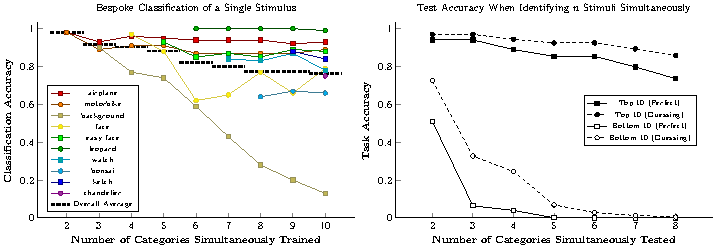
\includegraphics[width=\linewidth]{Figure-01.pdf}% This is a *.jpg file
%\end{center}
% \textbf{\refstepcounter{figure}\label{fig:01} Figure \arabic{figure}.}{ Performance of the bag-of-features classifier using 100 feature clusters. (Left) Classification accuracy given training on the ten largest categories in the Caltech 101 sample set. Colored lines show accuracy for specific categories, while dashed black lines show overall accuracy for each level of training complexity. (Right) Accuracy by a classifier trained on 102 categories during a test in which $n$ stimuli must be classified correctly for a trial to be `correct.' Performance for the classifier's ten best (black) and worst (white) categories was gauged. Solid lines indicate cases in which classification was done perfectly, while dashed lines indicate cases where correct responses required at least one guess.}
%\end{figure}

\subsection*{Training a Bespoke Classifier}

The ten largest image categories in the Caltech 101 set were set aside. The classifier was trained and subsequently validated using the first two of these categories, then the first three, and so forth up to ten. Because the classifier was limited to 100 clusters, its criteria became more general as the number of categories increased. The accuracy for each category, as well as the overall average, is plotted in Figure 1 (left).

Some image categories continue to perform well as additional categories are added: Airplanes, leopards, and `easy' faces were categorized correctly over 85\% of the time. However, other categories did less well when the classifier was forced to generalize, and in particular, the category of `background images' became steadily harder to classify, presumably due to the lack of consistent discrete features. If this algorithm was being studied with only three categories, however, this deficiency would not be apparent: Backgrounds were categorized correctly 90\% of the time when competing with only two other possible choices.

\subsection*{Measuring the Benefits of Guessing}

We retrained the classifier using all 102 image categories in parallel. The classifier was then tested using the following procedure: Exactly one novel image was drawn from each of $n$ categories, and the classifier had to match \textsl{every} image with its corresponding category. If the classifier judged more than one stimulus to belong to a given category, it guessed. In the four-category test, for example, a total of four responses were required to complete the trial.

Figure 1 (right) shows performance when the classifier's ten best categories (black) and ten worst categories (white) were tested in this way. Solid lines show the trials in which every stimulus was correctly identified without guessing, while dashed lines show those trials that were correct given at least one guess. Although there is a clear distinction between high and low performance, there is always a benefit for guessing. In the two-item test, a poor classifier guessed its way to 72\% accuracy, a level that would be considered `high' in many published studies. In three- and four-category tests, almost every correct trial for the poor classifiers involved at least some guessing.

\section*{Recommendations}

Our simulation makes clear the perils of overly narrow category training and overly simplistic tests. When a subject (or an algorithm) is trained on only a handful of categories, the resulting learning is likely to be overspecialized and fails to capture the classifier's general aptitudes. Similarly, when even a highly generalized classifier is tested on only a handful of categories at a time, a considerable number of correct trials may result from informed guessing rather than from having a robust representation of all the extent categories.

In our simulation, we demonstrate these problems separately, but the two can easily act in concert. A study that uses \textsl{only} two categories throughout training and testing may elicit learning, but it is nearly impossible to judge whether the result arises from any abstract understanding of the stimuli. 

The best defense against the possibility of a bespoke classifier is to increase the number of categories that are trained in parallel. While various clever tricks may permit pictures of faces to be distinguished from pictures of houses, such trickery is more difficult given three categories, still more difficult given four, and so on. This is especially true if subjects do not show a monotonic increase in reaction times as the number of trained categories increases.

Many studies that trained more than two categories \citep[e.g.][]{Herr1976, Siga2009, Vonk2013} still test only one stimulus at a time. Other studies have required that subjects match a stimulus to one of four categories \citep{Bhat1988, Laza2004}. Although an improvement, such match-to-sample procedures still frequently reward guessing.

Contrary to the recommendations of \citet{Katz2007}, we recommend that test conditions require subjects to identify more than one stimulus category during each trial. Unfortunately, few validated methods provide an appropriate level of response complexity. One candidate is the simultaneous chain \citep{Terr2005}, which has been used to test serial and numerical cognition. Another candidate is the ALVIN procedure \citep{Wash1995}, albeit adapted to using novel categorical stimuli. Recovering from the weaknesses of prior concept studies will require that researchers raise the bar, and give their animal subjects the opportunity to succeed (or fail) on their own cognitive merits.

\section*{Disclosure/Conflict-of-Interest Statement}

The authors declare that the research was conducted in the absence of any commercial or financial relationships that could be construed as a potential conflict of interest.

\section*{Author Contributions}

GJ and DA both contributed the conceptualization, analysis, and writing of this piece.

\section*{Acknowledgement}
The author wish to thank [insert names here]. [Funding]

\bibliography{binar_refs}

\end{document}
